\documentclass{article}
% Load packages
\usepackage{tikz} % to draw neural network
\usepackage{lscape}
\usepackage{graphicx}   % Including figure files
\thispagestyle{empty}
\begin{document}
%\begin{landscape}
%\begin{figure}
%    \centering
%    \includegraphics[width=\textwidth]{eboss-dr7.png}
%    \includegraphics[width=\textwidth]{corrmax-dr7.pdf}
%\end{figure}

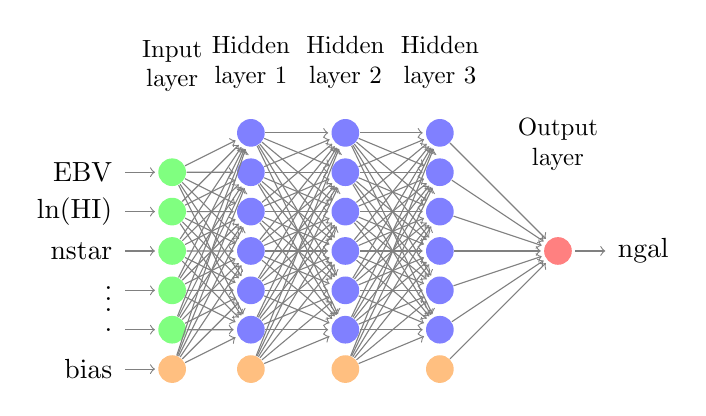
\begin{tikzpicture}[shorten >=1pt,->,draw=black!50, node distance=1.5cm]
    \tikzstyle{every pin edge}=[<-,shorten <=1pt]
    \tikzstyle{neuron}=[circle,fill=black!25,minimum size=10pt,inner sep=0pt]
    \tikzstyle{input neuron}=[neuron, fill=green!50];
    \tikzstyle{output neuron}=[neuron, fill=red!50];
    \tikzstyle{hidden neuron}=[neuron, fill=blue!50];
    \tikzstyle{bias neuron}=[neuron, fill=orange!50];
    \tikzstyle{annot} = [text width=4em, text centered, scale=0.9]
    % Draw the input layer nodes
    \foreach \name / \y in {EBV/1, ln(HI)/2, nstar/3, \vdots/4, ./5}
        \node[input neuron, pin=left:\name] (I-\y) at (0,-0.5*\y) {};
    \node[bias neuron, pin=left:bias] (I-6) at (0,-3.) {};         
    % Draw first hidden layer nodes
    \foreach \name / \y in {1,...,6}
        \path[yshift=0.5cm]
            node[hidden neuron] (H-\name) at (1.0 cm,-0.5*\y cm) {}
            node[hidden neuron] (G-\name) at (2.2 cm,-0.5*\y cm) {}    
            node[hidden neuron] (L-\name) at (3.4 cm,-0.5*\y cm) {};                        
    \node[bias neuron] (H-7) at (1.0 cm,-3. cm) {};
    \node[bias neuron] (G-7) at (2.2 cm,-3. cm) {};            
    \node[bias neuron] (L-7) at (3.4 cm,-3. cm) {};
     % Draw the output layer node
    \node[output neuron,pin={[pin edge={->}]right:ngal}, right of=L-4] (O) {};
    % connect nodes
    \foreach \source in {1,...,6}
        \foreach \dest in {1,...,6}
            \path (I-\source) edge (H-\dest);
    \foreach \source in {1,...,7}
        \foreach \dest in {1,...,6}
            \path (H-\source) edge (G-\dest);
    \foreach \source in {1,...,7}
        \foreach \dest in {1,...,6}
            \path (G-\source) edge (L-\dest);
     % Connect every node in the hidden layer with the output layer
    \foreach \source in {1,...,7}
        \path (L-\source) edge (O);
     % Annotate the layers
    \node[annot,above of=I-1] {Input layer};
    \node[annot,above of=H-1, node distance=1.0 cm] (hl1) {Hidden layer 1};
    \node[annot, above of=G-1, node distance=1.0 cm] (hl2) {Hidden layer 2};
    \node[annot, above of=L-1, node distance= 1.0 cm] (hl3){Hidden layer 3};
    \node[annot,above of=O] {Output layer};    
\end{tikzpicture}
%\end{landscape}
\end{document}

